\subsection{Error Detection and Correction}
One of the big challenges of physically realising a quantum 
computer is its subjection to noise in the real world.
Unlike classical computers, the type of error is not limited
to a bitflip, as even single qubit states have a theoretically
infinite amount of differing states to it on a bloch sphere,
and therefore an infinite amount of types of errors can have
occured in the presence of noise such as thermal or electromagnetical
noise.

Fortunately, this noise can be modeled as successive pauli gates.
Since an identity noise occuring is irrelevant to us, and XY as
well as ZY (anti-) commute, we need only correct for X and Z
errors occuring in order to correct any pauli errors. 

\subsubsection{Repetition Code}
In order to correct errors, they must first be detected.
From classical computer science there are well known existing
codes, such as the repetition code.
For this error code information is encoded by repeating the 
intended message some amount of times, and then decoding it
by performing a majority vote on the transmitted message.
In Quantum error correction, we speak of [[n,k,d]] stabilizer
codes if an encoding scheme allows for n physical qubits to 
encode k logical qubits to a distance d.

\begin{figure}[h!]
	\begin{center}
	\captionsetup{justification=centering,margin=2cm}
	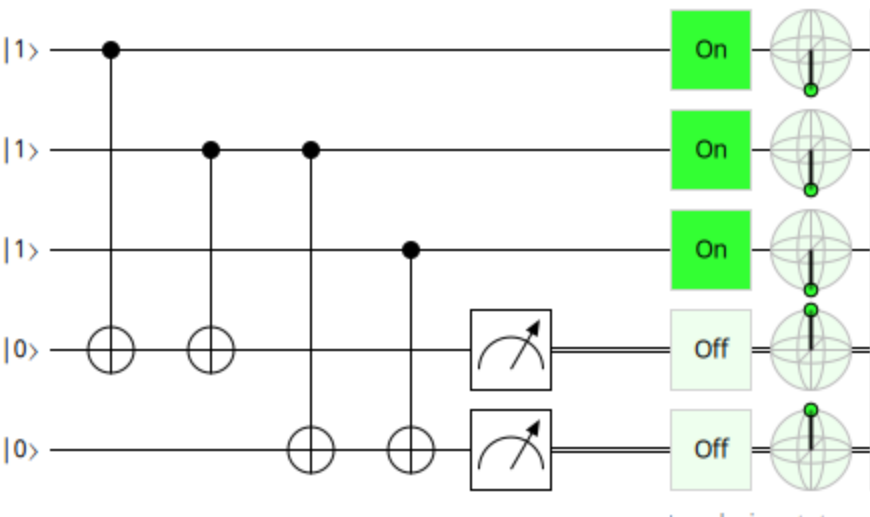
\includegraphics[scale=0.2]{./img/bitflipSyndromeExtraction3Rep.png}\\
	\caption{Bitflip Syndrome extractor\\
        +1 measurement result on first Ancilla indicates a bitflip error
        on qubits 1 or 2, +1 result on second ancilla indicates 
		bitflip on second or third qubit}
	\label{fig: syndrome extractor}
	\end{center}
\end{figure}

A quantum equivalent of the 3-bit repetition code performed on
the message $|1\rangle$ is is the [[3,1,$\frac{1}{2}$]] repetition
code depicted in 
figure~\ref{fig: syndrome extractor}, including so-called
``Syndrome Extraction''. A Syndrome is a stabilizer that can be
measured in order to detect wether and where an error has occured
in a multi-qubit system. It is crucial that the 
measurement of such Syndromes occurs without harming the actual
quantum information stored in the ``data-qubits''. Therefore
two additional ``Ancilla-qubits'' (both initialized to 
$|0\rangle$) are attached to the circuit via CNOTs.
This circuit is stabilized by IZZ and ZZI, measured by ancilla 
1/2. The measurement result will therefore be a vector of length
two, with each entry either being +1 or -1. To simplify the 
algebra this will be changed to the binary representation of 0 
for +1 and 1 for -1. 

To represent the code, Stabilizers can be stacked together to
a so-called parity-check-matrix, which satisfies:
\begin{equation}
	M_{pc}\cdot \vec{v}_{error} = \vec{v}_{syndrome}
\end{equation}
So e.g. the parity check matrix for the $[3,1,\frac{1}{2}]$
repetition code would be:

\begin{equation}
	M_{pc3} = \left( 
	\begin{array}{ccc}
		1 & 1 & 0 \\
		0 & 1 & 1
	\end{array}
	\right)
\end{equation}
And the syndrome for an X error on the first qubit would be
$\left(\begin{array}{c}1\\0\end{array}\right)$.

This way of encoding information however leaves two notable
issues:

For one, it only detects bitflip, or pauli-X errors occuring on
the stored quantum information. While using Hadamard gates one
could trivially adapt this code to instead detect pauli-Z errors,
it is not possible to use linear codes like the repetition code
to $simultaneously$ detect pauli-X and pauli-Z errors occuring.

Secondly, it also assumes a noise model of a ``Noisy Channel'',
which is not compatible with the actually encountered errors in
real physical quantum computers.
\newpage
\subsubsection{2D Codes}
Previous research in computer science 
provides a toolset for generating valid codes
from existing encoding schemes. 
Hypergraph product codes, introduced by Tillich and Z\'emor,
of two 
existing codes will always remain a valid detection code.
We can therefore form a hypergraph product code of two repetition
codes for X error detection and Z error detection respectively,
obtaining the [[$d^2$,1,d]]``Surface-Code'' which can detect up
to d of $both$ X and Z errors, and 
therefore any pauli error happening.

The parity check matrix of a hypergraph product code is generated
by the parity check matrices of two valid codes in the following
way:
\begin{equation}
	H = \left(\begin{array}{cc}
		M_{pcX} & 0 \\
		0 & M_{pcZ} \\
	\end{array}\right)
\end{equation}

PUT IN A NICE VISUALISATION OF THE SURFACE CODE.
